\section{Statistiken}

Über die 4 Wochen Implementierungsdauer wurden ungefähr 5000 Zeilen Code geschrieben.
Dabei gab es über 240 Commits von 4 Accounts.
Die Aufgaben waren wie zuvor auch nach Anwendungsbereich sortiert. Durch die teilweise Überlappung
mit einer Klausurvorbereitung erfolgten in den ersten zwei Wochen erheblich mehr Commits als in 
den späteren. Dies stellt allerdings kein Problem dar da dies von Anfang an bekannt
und auch einkalkuliert war.\\

Die internen Statistiken von Git sind bei React kaum benutzbar da die package-lock.json
zeilenmäßig den Großteil der Anwendung einnimmt und automatisch generiert wird.
Laut NPM ist diese Datei aber im Repository erforderlich.

Commitanzahl über Zeit, laut GitHub\\
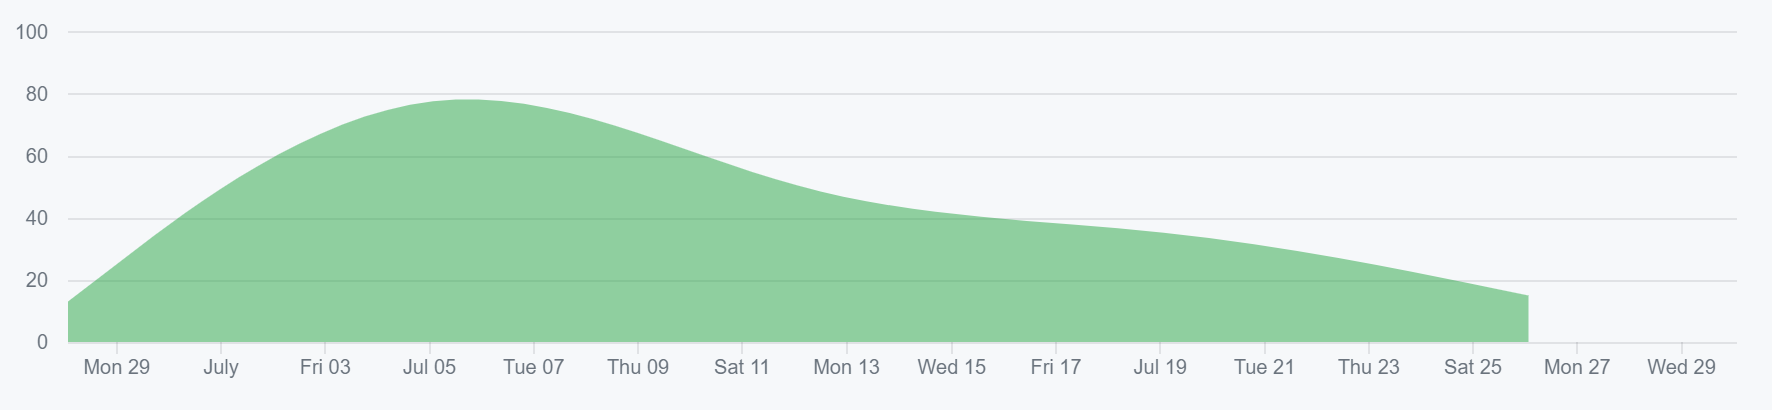
\includegraphics[width=\textwidth]{Commits.png}